\documentclass[a4paper,12pt]{article}
\usepackage[utf8]{inputenc}
\usepackage[spanish]{babel}
\usepackage{amsmath}
\usepackage{amsfonts}
\usepackage{graphicx}
\usepackage{booktabs}
\usepackage{placeins}
\usepackage{hyperref}
\usepackage{fancyhdr}
\usepackage[a4paper, left=2.5cm, right=2.5cm, top=2.5cm, bottom=2.5cm]{geometry}

\begin{document}
\begin{titlepage}
    \fancypagestyle{portraitstyle}{
        \fancyhf{}
        \fancyhead[L]{
            
\includegraphics[height=2cm]{/img/departamentos/fiudec.pdf}
        }
        \fancyhead[R]{
            
\includegraphics[height=2cm]{/img/departamentos/fiudec2.pdf}
        }
    }
    \centering
    \vspace*{3cm}
    
    {\Huge \textbf{Proyecto Semestral}}\\[1cm]
    
    {\LARGE Análisis comparativo de TowerSketch y Count-Min Sketch multinivel: Evaluación de precisión}\\[3cm]
    
    \vfill
    \begin{flushright}
        \textbf{Nombre:} \\
        Roberto Artigues Escobar \\[1cm]
        
        \textbf{Matrícula:} \\
        2019082094 \\[1cm]
        
        \textbf{Docente:} \\
        Cecilia Hernández
    \end{flushright}
    
    \vfill
    TOPICOS EN MANEJO DE GRANDES VOLUMENES DE DATOS 503302-1 
\end{titlepage}

\tableofcontents
\newpage

\section{Resumen}
El monitoreo de flujos de red es fundamental para la gestión y seguridad de las redes modernas. Este trabajo presenta un análisis comparativo entre dos estructuras de datos probabilísticas: TowerSketch y una implementación multinivel del Count-Min Sketch.
Utilizando datos reales de CAIDA, se evalúa el rendimiento de ambos esquemas en términos de precisión y eficiencia de memoria. \\ \\ Los resultados demuestran la superioridad significativa de TowerSketch, alcanzando errores relativos cercanos a cero con mayores cantidades 
de memoria, mientras que el Count-Min Sketch multinivel mantiene errores más elevados incluso en condiciones óptimas. Este estudio proporciona evidencia empírica sobre las ventajas de la estructura jerárquica de TowerSketch para el monitoreo eficiente de flujos de red.

\section{Introducción}
\subsection{Contexto y Motivación}
En el contexto actual de las redes de computadores, el monitoreo eficiente de flujos de red se ha convertido en un desafío crítico debido a:

\begin{itemize}
    \item El crecimiento exponencial del volumen de tráfico de red
    \item La necesidad de procesar y analizar datos en tiempo real
    \item Las limitaciones de memoria en dispositivos de red
    \item Los requerimientos de alta precisión en la estimación de estadísticas
\end{itemize}

Las estructuras de datos probabilísticas han emergido como una solución prometedora para estos desafíos, ofreciendo un compromiso entre precisión y uso de memoria. Existen propuestas recientes que han demostrado ventajas significativas en términos de eficiencia y precisión, como TowerSketch, que utiliza una estructura jerárquica para mejorar la estimación de flujos. 

\subsection{Objetivos}
Este trabajo tiene como objetivos principales:

\begin{itemize}
    \item Realizar un análisis comparativo exhaustivo entre TowerSketch y una implementación multinivel del Count-Min Sketch
    \item Evaluar el rendimiento de ambas estructuras bajo diferentes configuraciones de memoria
    \item Analizar la precisión en la estimación de flujos tanto frecuentes como infrecuentes
\end{itemize}

\subsection{Alcance}
El estudio se centra en:

\begin{itemize}
    \item Implementación y evaluación de TowerSketch y Count-Min Sketch multinivel
    \item Análisis utilizando trazas de red reales de CAIDA
    \item Evaluación comparativa de métricas de error relativo y absoluto
    \item Comparación del comportamiento con diferentes configuraciones de memoria (4KB a 64MB)
\end{itemize}

\newpage
\section{Marco Teórico}
\subsection{Sketches Probabilísticos}
Los sketches probabilísticos son estructuras de datos que permiten estimar estadísticas sobre grandes conjuntos de datos utilizando memoria sublineal. Sus principales características incluyen:

\begin{itemize}
    \item Uso de memoria constante independiente del tamaño de entrada
    \item Garantías probabilísticas de error
    \item Trade-off ajustable entre precisión y uso de memoria
\end{itemize}

\subsection{TowerSketch}
TowerSketch representa un avance significativo en el diseño de sketches probabilísticos, implementando una estructura jerárquica innovadora:

\begin{itemize}
    \item Estructura de múltiples niveles con tamaños de contador optimizados
    \item Cada nivel utiliza $2^{i+1}$ bits por contador, donde i es el nivel
    \item Funciones hash independientes por nivel para mejor distribución
    \item Empaquetamiento eficiente de contadores en palabras de 32 bits
\end{itemize}

La eficacia de TowerSketch se basa en:
\begin{itemize}
    \item Minimización de colisiones mediante múltiples niveles
    \item Optimización del espacio mediante contadores de tamaño variable
    \item Estimación precisa basada en el mínimo valor entre niveles
    \item Balance eficiente entre precisión y uso de memoria
\end{itemize}

\subsection{Count-Min Sketch Multinivel}
El Count-Min Sketch multinivel es una extensión del CM tradicional que introduce:

\begin{itemize}
    \item Múltiples niveles con diferentes capacidades de conteo
    \item Sistema de promoción basado en umbrales
    \item Seguimiento del nivel actual de cada elemento
    \item Altura fija por nivel para maximizar filas de contadores
\end{itemize}

La estructura implementa:
\begin{equation}
    \text{Promoción si: } valor\_contador \geq umbral\_nivel \times factor\_overflow
\end{equation}

Aunque este enfoque busca mejorar la precisión mediante la separación de flujos, los resultados experimentales demuestran que TowerSketch logra una mejor eficiencia general en términos de precisión y uso de memoria.

\begin{figure}[h]
    \centering
    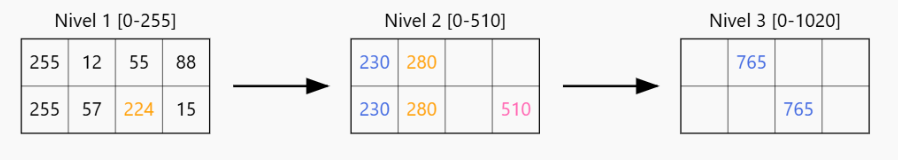
\includegraphics[width=0.9\textwidth]{img/ml-cm.png}
    \caption{Estructura de ejemplo, Count-Min Sketch multinivel}
\end{figure}

\newpage
\section{Metodología}
\subsection{Diseño Experimental}
El experimento fue diseñado para realizar una comparación exhaustiva entre TowerSketch y Count-Min Sketch multinivel (MCM) bajo condiciones controladas. El entorno experimental consistió en:

\begin{itemize}
    \item \textbf{Hardware}:
    \begin{itemize}
        \item Procesador: Intel(R) Core(TM) Ultra 7 165H (22) @ 5.00 GHz
        \item Memoria RAM: 32 GB
    \end{itemize}
    
    \item \textbf{Parámetros de Evaluación}:
    \begin{itemize}
        \item Rango de memoria: 4KB a 64MB
        \item Número de ejecuciones por configuración: 10 (REP\_TIME)
        \item Máximo de paquetes procesados: 20 millones
        \item Factor de overflow para MCM: 0.50
    \end{itemize}
\end{itemize}

\subsection{Configuración de Estructuras}
\subsubsection{TowerSketch}
\begin{itemize}
    \item \textbf{Parámetros Estructurales}:
    \begin{itemize}
        \item Número de niveles (d): 5
        \item Bits por contador por nivel: [2, 4, 8, 16, 32] bits
        \item Máscaras de nivel: [0x3, 0xf, 0xff, 0xffff, 0xfffff]
    \end{itemize}
    
    \item \textbf{Características por Nivel}:
    \begin{itemize}
        \item Bits de desplazamiento (cs): [1, 2, 3, 4, 5]
        \item Contadores por palabra (cpw): [4, 3, 2, 1, 0]
        \item Máscaras de bit bajo (lo): [0xf, 0x7, 0x3, 0x1, 0x0]
    \end{itemize}
\end{itemize}

\subsubsection{Count-Min Multinivel}
\begin{itemize}
    \item \textbf{Parámetros Estructurales}:
    \begin{itemize}
        \item Profundidad (ML\_DEPTH): 5 niveles
        \item Altura fija (ML\_HEIGHT): 5 filas
        \item Bits por contador por nivel: [2, 4, 8, 16, 32] bits
        \item Máscaras de nivel: [0x3, 0xf, 0xff, 0xffff, 0xfffff]
    \end{itemize}
    
    \item \textbf{Características por Nivel}:
    \begin{itemize}
        \item Bits de desplazamiento (ML\_CS): [1, 2, 3, 4, 5]
        \item Contadores por palabra (ML\_CPW): [4, 3, 2, 1, 0]
        \item Máscaras de bit bajo (ML\_LO): [0xf, 0x7, 0x3, 0x1, 0x0]
    \end{itemize}
\end{itemize}

\subsection{Conjuntos de Datos}
Se utilizó el dataset CAIDA 2018 como fuente principal de datos:

\begin{itemize}
    \item \textbf{Características del Dataset}:
    \begin{itemize}
        \item Formato: Registros binarios de 13 bytes por flujo
        \item Tamaño: 20 millones de paquetes
        \item Identificación: Tuplas únicas de 13 bytes por flujo
    \end{itemize}
\end{itemize}

\subsection{Métricas de Evaluación}
Se implementaron cuatro métricas principales:

\begin{itemize}
    \item \textbf{Error Relativo Promedio (ARE)}:
    \begin{equation}
        ARE = \frac{1}{n}\sum_{i=1}^{n}\frac{|e_i - t_i|}{t_i}
    \end{equation}
    
    \item \textbf{Error Absoluto Promedio (AAE)}:
    \begin{equation}
        AAE = \frac{1}{n}\sum_{i=1}^{n}|e_i - t_i|
    \end{equation}
    
    \item \textbf{Tasa de Utilización de Contadores}:
    \begin{equation}
        \text{Utilización} = \frac{\text{Contadores\_Usados}}{\text{Total\_Contadores}} \times 100
    \end{equation}
    
    \item \textbf{Análisis por Percentiles}:
    \begin{itemize}
        \item Separación de flujos al 80º percentil
        \item Evaluación independiente de ARE y AAE por grupo
    \end{itemize}
\end{itemize}

\subsection{Implementación de Funciones Hash}
Ambas estructuras utilizan MurmurHash3 para el mapeo de flujos:
\begin{itemize}
    \item Semillas aleatorias independientes por nivel
    \item Distribución uniforme para minimizar colisiones
\end{itemize}

\subsection{Recolección de Datos}
El proceso experimental genera cuatro archivos de resultados:

\begin{itemize}
    \item \texttt{sketch\_results.csv}: Métricas generales ARE/AAE
    \item \texttt{percentile\_results.csv}: Análisis por tipo de flujo
    \item \texttt{tower\_level\_info.csv}: Estadísticas de TowerSketch
    \item \texttt{mcm\_level\_info.csv}: Estadísticas de MCM
\end{itemize}

\newpage 
\section{Resultados}

Los resultados detallados del experimento, incluyendo gráficos interactivos y tablas completas, están disponibles en \url{graficos.oracle.rartigues.com}. A continuación, se presenta un análisis de los datos obtenidos.

\subsection{Análisis de Precisión}
\noindent El análisis de precisión se realizó mediante la evaluación del Error Relativo Promedio (ARE) y Error Absoluto Promedio (AAE) para diferentes configuraciones de memoria:

\begin{itemize}
    \item \textbf{Comportamiento General}: TowerSketch muestra una mejora significativa en precisión con el aumento de memoria, alcanzando un ARE de 0.00002\% con 64MB, mientras que MCM mantiene un error más alto de 8.13\%.
    
    \item \textbf{Escalabilidad}: Los resultados muestran que TowerSketch escala mejor con el aumento de memoria:
\begin{itemize}
    \item Con 4KB: TowerSketch ARE $\approx$ 30.597\%, MCM ARE $\approx$ 26.965\%
    \item Con 64MB: TowerSketch ARE $\approx$ 0.00002\%, MCM ARE $\approx$ 8.13\%
\end{itemize}

\item \textbf{Error Absoluto}: El AAE sigue un patrón similar, con TowerSketch mostrando una reducción más pronunciada del error al aumentar la memoria.
\end{itemize}

\subsection{Análisis por Tipos de Flujo}
El análisis de percentiles revela comportamientos distintos para flujos frecuentes e infrecuentes:

\begin{itemize}
    \item \textbf{Flujos Frecuentes}:
    \begin{itemize}
        \item TowerSketch muestra mejor rendimiento en general
        \item La diferencia se acentúa con mayor memoria disponible
        \item Convergencia más rápida hacia errores bajos
    \end{itemize}
    
    \item \textbf{Flujos Infrecuentes}:
    \begin{itemize}
        \item Ambas estructuras muestran errores más altos
        \item TowerSketch mantiene ventaja en precisión
        \item Mayor variabilidad en las estimaciones
    \end{itemize}
\end{itemize}

\subsection{Análisis de Uso de Niveles}
El comportamiento de los niveles muestra patrones distintivos:

\subsubsection{TowerSketch}
\begin{itemize}
    \item Distribución gradual de la utilización entre niveles
    \item Reducción progresiva del uso de niveles inferiores con mayor memoria
    \item Mejor balance en la utilización de contadores entre niveles
\end{itemize}

\subsubsection{CM-Multinivel}
\begin{itemize}
    \item Alta concentración en niveles superiores
    \item Caída abrupta en la utilización del nivel 4 (32-bit)
    \item Menor eficiencia en la distribución de contadores
\end{itemize}

\subsection{Eficiencia de Memoria}
El análisis de eficiencia de memoria muestra que:

\begin{itemize}
    \item TowerSketch logra mejor utilización del espacio disponible
    \item La estructura jerárquica de TowerSketch permite una mejor adaptación a diferentes patrones de tráfico
    \item MCM muestra saturación más rápida de niveles superiores
\end{itemize}

\subsection{Hallazgos Clave}
Los resultados principales del estudio son:

\begin{itemize}
    \item TowerSketch supera consistentemente a MCM en precisión, especialmente con mayor memoria disponible
    \item TowerSketch maneja mejor tanto flujos frecuentes como infrecuentes
    \item La distribución de contadores es más eficiente en TowerSketch
\end{itemize}

\noindent Se realizaron los experimentos con datos autogenerados con sesgo y sin sesgo, y se encontró que TowerSketch mantiene una precisión superior en ambos casos, lo que sugiere una mayor robustez en entornos reales.

\newpage
\section{Conclusiones}

Este estudio comparativo entre TowerSketch y Count-Min Sketch multinivel revela diferencias significativas en rendimiento y diseño estructural. TowerSketch demostró superioridad en términos de:

\begin{itemize}
    \item \textbf{Precisión}: Mejores resultados tanto en ARE como AAE, especialmente con memoria superior a 1MB, alcanzando errores cercanos a cero con 64MB mientras CM-Multinivel mantiene errores superiores al 8\%.
    
    \item \textbf{Eficiencia Estructural}: La distribución jerárquica de TowerSketch (32,768 contadores en nivel base para 256KB) permite un mejor aprovechamiento de memoria que la distribución uniforme de CM-Multinivel (257x51 por nivel).
    
    \item \textbf{Manejo de Flujos}: Mayor efectividad tanto en flujos frecuentes como infrecuentes, evidenciado en el análisis por percentiles.
\end{itemize}

Las principales limitaciones identificadas incluyen:
\begin{itemize}
    \item CM-Multinivel subutiliza sus niveles superiores
    \item Ambas estructuras muestran sensibilidad con memoria inferior a 16KB
    \item CM-Multinivel requiere más contadores totales (65,535 vs 63,488 en 256KB) para un rendimiento inferior
\end{itemize}

\section{Trabajo Futuro}
\noindent Cualquier trabajo futuro en Multilevel Count-Min Sketch debería considerar las siguientes áreas de mejora:
\begin{itemize}
    \item Optimizar la utilización de memoria en CM-Multinivel
    \item Evaluar el rendimiento con diferentes datasets
    \item Investigar umbrales de promoción alternativos
\end{itemize}

\noindent La arquitectura actual de ML CM no logra aprovechar eficientemente la memoria disponible, lo que sugiere la necesidad de un rediseño estructural para mejorar su rendimiento.

\newpage

\begin{thebibliography}{9}

\bibitem{towersketch}
Yang, T., Yang, H., Liu, A. X., Meng, J., Sha, Z., \& Li, B. (2021).
\emph{TowerSketch: A compressed sketch for better heavy-hitter identification}.
In 2021 IEEE 29th International Conference on Network Protocols (ICNP) (pp. 1-11).
IEEE.

\end{thebibliography}

\appendix
\section{Código Fuente}
\noindent Todo el código fuente utilizado en este trabajo se encuentra disponible en el repositorio de GitHub: \url{https://github.com/rartigues/ProyectoVolumDatos}.
Detalle acerca de la implementación del proyecto se encuentra en el archivo README.md.

\end{document}